\chapter{Java mit SQL -- Wiederholung}
\renewcommand{\chaptertitle}{Java mit SQL -- Wiederholung}

\lehead[]{\normalfont\sffamily\hspace*{-2.00cm}\textcolor{white}{\colorbox{lightblue}{\parbox[c][0.70cm][b]{1.60cm}{
\makebox[1.60cm][r]{\thechapter}\\ \makebox[1.60cm][r]{ÜBUNG}}}}\hspace{0.17cm}\textcolor{lightblue}{\chaptertitle}}
\rohead[]{\textcolor{lightblue}{\chaptertitle}\normalfont\sffamily\hspace*{0.17cm}\textcolor{white}{\colorbox{lightblue}{\parbox[c][0.70cm][b]{1.60cm}{\thechapter\\
ÜBUNG}}}\hspace{-2.00cm}}
%\chead[]{}
\rehead[]{\textcolor{lightblue}{AvHG, Inf, My}}
\lohead[]{\textcolor{lightblue}{AvHG, Inf, My}}

\section*{Klausurvorbereitung}

\subsection{Aufgabe 1: Umwandlung von Strings in Zahlen}

\begin{compactenum}[a)]
\item Schreibe den Text aus dem JTextField \myUserInput{eingabe} in eine
String-Variable und konvertiere ihn anschließend in eine Integer-Zahl.
\item Was passiert, wenn in dem Textfeld gar keine Zahl stand? Erweitere den
Code-Auszug so, dass gegebenenfalls eine Fehlermeldung auf der Konsole
ausgegeben wird.
\end{compactenum}


\subsection{Aufgabe 2: String-Vergleich}

\begin{compactenum}[a)]
\item Gegeben sind die String-Variablen \myUserInput{text1} und
\myUserInput{text2}. Frage ab, ob in beiden Variablen der selbe Text steht und
gib auf der Konsole eine Erfolgsmeldung oder eine Fehlermeldung aus.
\item Wie muss man den Code-Auszug verändern, wenn die Groß- und Kleinschreibung
bei der Abfrage auf Gleichheit keine Rolle spielen soll?
\end{compactenum}


\subsection{Aufgabe 3: Programmierübung zur Haustier-Datenbank}

Programmiere zur Übung noch einmal eine kleine Anwendung, die sich auf die
Haustier-Datenbank bezieht. Verwende bei der Erstellung des Programms
ausschließlich die in der Klausur erlaubten Merkblätter!

\begin{center}
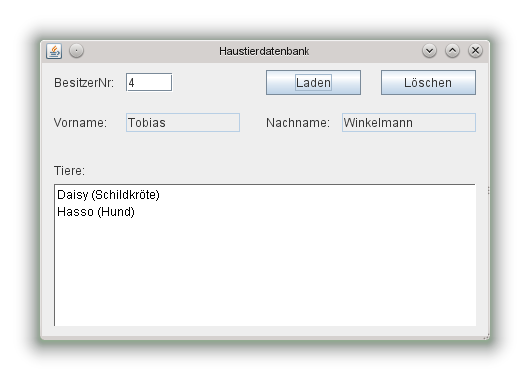
\includegraphics[width=0.65\textwidth]{./inf/SEKII/38_JavaSQL_Wiederholung/HaustierdatenbankAufgabe3.png}
\end{center}

Die Textfelder zur Ausgabe des Vornamens und Nachnamens des Besitzers sollen
nicht editierbar sein. In der JList-Komponente sollen nur die lebendigen Tiere
des jeweiligen Besitzers aufgelistet werden. Falls ein Besitzer mit der
angegebenen BesitzerNr nicht existiert, soll eine Fehlermeldung ausgegeben
werden.

Nach dem Löschen eines Besitzers soll eine Erfolgs- oder Fehlermeldung
ausgegeben werden. Der Inhalt der Textfelder und der JList-Komponente soll beim
erfolgreichen Löschen eines Besitzers ebenfalls gelöscht werden.

Der Rest sollte selbsterklärend sein.


\subsection{Aufgabe 4: KFZ-Werkstatt}

Es soll eine Anwendung für die KFZ-Werkstätten erstellt werden, in der die zur
Reparatur oder Wartung gegebenen Fahrzeuge verwaltet werden. In dieser Datenbank
sollen sich nur Fahrzeuge und Aufträge befinden, die am aktuellen Tag noch
bearbeitet werden müssen. Alle bearbeiteten Aufträge werden sofort aus der
Datenbank gelöscht.

Ein Kollege von dir hat bereits die SQL-Anweisungen zur Erstellung einer
geeigneten Datenbank (inklusive Testdaten) geschrieben. Du findest die
SQL-Anweisungen in der Datei \myFile{werkstatt.sql} auf. Erzeuge mit Hilfe
dieser Datei eine neue Datenbank auf deinem Computer.

\begin{compactenum}[a)]
\item Analysiere die Datenbank und zeichne ein ER-Diagramm, das die Struktur der
 Datenbank darstellt.
\item Gib an, in welcher Normalform sich die Datenbank \myUserInput{werkstatt}
befindet. Begründe deine Antwort.
\item Später soll ein Computerprogramm erstellt werden, das den Mitarbeitern der
KFZ-Werkstatt eine einfache Bedienoberfläche für die Datenbank liefert.
Formuliere als Vorbereitung dafür geeignete Datenbank-Abfragen, mit denen die
folgenden Informationen aus der Datenbank \myUserInput{werkstatt} gewonnen
werden können. Speichere die SQL-Abfragen in einer Datei auf dem USB-Stick ab.

\begin{compactenum}[1.]
\item Liste Vor- und Nachname aller Mechaniker auf, die das Fahrzeug mit der
Nummer 2 bearbeiten.
\item Liste alle Fahrzeuge mit ihrer Fahrzeug-Nummer auf, die der Mechaniker
Karl Sonntag zu bearbeiten hat.
\item Liste Fahrzeug-Nummer und Typ derjenigen Fahrzeuge auf, die noch vor 16
Uhr fertig werden müssen.
\item Ein Auftrag hat länger gedauert als erwartet und die versprochenen Zeiten
können nicht eingehalten werden. Die Kunden müssen darüber informiert werden,
dass sie ihre Fahrzeuge erst später abholen können. Liste alle Daten der Kunden
auf, deren Fahrzeuge bis einschließlich 17 Uhr fertig werden sollten. Es sollen
keine Kunden doppelt in der Liste erscheinen. Sortiere die Liste aufsteigend,
zuerst nach dem Nachnamen und dann nach dem Vornamen der Kunden.
\item Liste alle Fahrzeuge mit Fahrzeug-Nummer auf, bei denen zwei oder mehr
Tätigkeiten durchgeführt werden müssen.
\item Liste alle Fahrzeuge mit ihrer Fahrzeug-Nummer auf, die zur selben Zeit
fertig werden müssen wie das Fahrzeug mit der Nummer 4. Das Fahrzeug mit der
Nummer 4 soll nicht in der Liste erscheinen.
\end{compactenum}
\end{compactenum}


\subsection{Aufgabe 5: Programmierung einer Software für ein Reiseunternehmen}

Ein Reiseunternehmen möchte exklusive Studienreisen anbieten für Kleingruppen
von maximal zwölf Personen. Du hast die Aufgabe, den Prototyp für die Software
zur Buchung der Reisen zu programmieren.

\begin{compactenum}[a)]
\item Die Datenbank zur Speicherung der angebotenen Reisen und der Buchungen
wurde bereits von einem Kollegen erstellt. Im Kurs-Repository findest du die
Datei \myFile{exklusiv\_reisen.sql}. Erzeuge mit Hilfe dieser Datei eine neue
Datenbank auf deinem Computer und analysiere sie. Erstelle ein ER-Diagramm, das
die Struktur der Datenbank abbildet.
\item Erläutere die Bedeutung der drei Normalformen und gib an, in welcher
Normalform sich die Datenbank befindet.
\item Erstelle ein Java-Programm, mit dem Reisen gebucht und storniert werden
 können. Abbildung \ref{fig:exklusivreisen} zeigt, wie die Oberfläche des
 Programms aussehen soll.
 
 \begin{figure}[h]
 \centering
 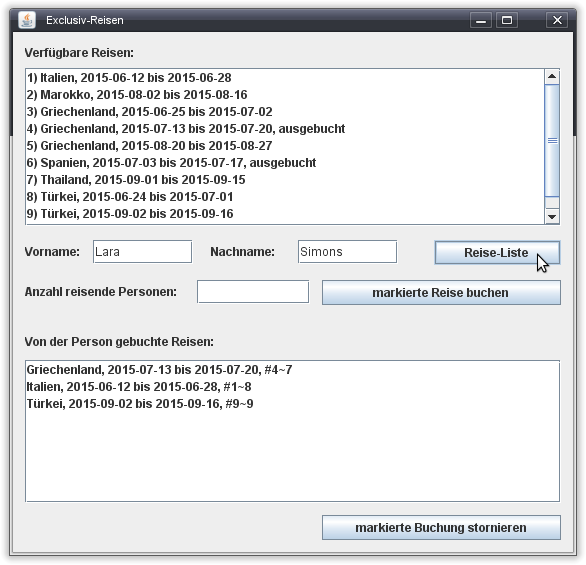
\includegraphics[width=0.85\textwidth]{./inf/SEKII/38_JavaSQL_Wiederholung/ExklusivReisenAufgabe5.png}
 \caption{Die Programmoberfläche von \glqq Exklusiv-Reisen\grqq}
 \label{fig:exklusivreisen}
 \end{figure}
 
In der oberen JList-Komponente werden alle verfügbaren Reisen aufgelistet. Schema:

\myUserInput{ReiseNr) Land, Anfangsdatum bis Enddatum}

Falls in der Spalte \myUserInput{ausgebucht} der Wert \myUserInput{ja} gesetzt
ist, wird zusätzlich die Zeichenkette "\myUserInput{, ausgebucht}" \ an den
Eintrag angehängt.

Wenn man auf den Button \myPMI{Reise-Liste} klickt, werden für die mit
Vornamen und Nachnamen angegebene Person alle gebuchten Reisen in der unteren
JList-Komponente aufgelistet. Es wird dabei vereinfacht davon ausgegangen, dass
es keine zwei Personen mit dem gleichen Vor- und Nachnamen geben kann. Die
Ausgabe der gebuchten Reisen erfolgt nach dem Schema:

\verb|Land, Anfangsdatum bis Enddatum, #ReiseNr~BuchungsNr|

Falls keine gebuchten Reisen gefunden werden, bleibt die JList-Komponente leer.
Es braucht keine Fehlermeldung ausgegeben werden.

Wenn man auf den Button \myPMI{markierte Buchung stornieren} drückt, wird die in
der unteren JList- Komponente selektierte Reise storniert. Falls keine Zeile in
der unteren JList-Komponente markiert ist, wird eine entsprechende
Fehlermeldung ausgegeben (z.B. "Bitte wählen Sie die Buchung aus, die storniert
werden soll."). Andernfalls wird die Buchung mit der angegebenen BuchungsNr gelöscht.
Außerdem wird in der Reise mit der angegebenen ReiseNr die Spalte ausgebucht
auf \myUserInput{nein} gesetzt, weil ja jetzt auf jeden Fall wieder ein
Reiseplatz verfügbar ist. Es muss nicht überprüft werden, ob die Reise zuvor
tatsächlich ausgebucht war oder nicht. Der Inhalt beider JList-Komponenten soll
nach dem Löschen automatisch aktualisiert werden. Eine Erfolgsmeldung muss
nicht ausgegeben werden.

Wenn man auf den Button \myPMI{markierte Reise buchen} drückt, wird für die mit
Vornamen und Nachnamen angegebene Person die in der oberen JList-Komponente
ausgewählte Reise für die angegebene Anzahl von Personen gebucht, sofern eine
Buchung möglich ist. Dazu wird zunächst geprüft, ob der Benutzer alle Angaben
korrekt vorgenommen hat. Falls eines der Textfelder leer ist oder im
Anzahl-Textfeld keine gültige Zahl steht (z.B. ein Buchstabe oder ein Wert der
kleiner als 1 ist), wird die Buchung mit einer entsprechenden Fehlermeldung
abgebrochen. Die Buchung wird ebenfalls mit einer Fehlermeldung abgebrochen,
wenn in der oberen JList-Komponente kein Eintrag selektiert wurde. Wenn die
Eingaben korrekt sind, muss überprüft werden, ob für die Reise noch die
gewünschte Anzahl von Plätzen verfügbar ist. Dies ist der Fall, wenn die
Gesamtzahl der Personen in allen Buchungen, die sich auf die Reise beziehen,
plus die Anzahl der gewünschten Plätze kleiner oder gleich zwölf ist. Falls die
Anzahl der verfügbaren Plätze nicht ausreicht, wird die Buchung mit einer
Fehlermeldung abgebrochen; andernfalls wird ein neuer Eintrag in die Tabelle
Buchung eingefügt.

Beachte dabei, dass die BuchungsNr von der Datenbank automatisch generiert
werden soll. Nachdem der neue Eintrag in die Datenbank eingefügt wurde, wird
die untere \myClass{JList}-Komponente aktualisiert, damit der Benutzer den
Erfolg der Buchung sieht. Falls die Reise nach Durchführung der Buchung ausgebucht ist
(also insgesamt zwölf Personen für die Reise gebucht sind), wird für die Reise
die Spalte ausgebucht in der Reisetabelle auf ja gesetzt. In diesem Fall muss
anschließend die obere JList-Komponente aktualisiert werden.
\end{compactenum}


\subsection{Aufgabe 6: Programmierung einer Software für einen Getränkehandel}

Du hast die Aufgabe, den Prototyp für die Software eines Getränkehandels zu
programmieren. Die Datenbank zur Speicherung der vorhandenen Getränke und der
Getränke-Lieferanten wurde bereits von einem Kollegen erstellt. Du findest die
SQL-Anweisungen in der Datei \myFile{getraenkehandel.sql} im Kurs-Repository.
Erzeuge mit Hilfe dieser Datei eine neue Datenbank auf deinem Computer.

\begin{compactenum}[a)]
\item Analysiere die Datenbank. Erstelle ein ER-Diagramm, das die Struktur der
Datenbank abbildet.

In der Tabelle \myUserInput{getränk} gibt es drei Spalten, die einer Erläuterung
bedürfen:

\begin{compactitem}
\item Die Spalte \verb|anzahl| gibt die Anzahl der Getränkekisten an, die
das Geschäft momentan vorrätig hat.
\item Die Spalte \verb|min_anzahl| gibt an, wie viele Kisten des Getränks sich
mindestens im Lager befinden sollten. Sobald die Anzahl der Getränkekisten
unter den Wert \verb|min_anzahl| sinkt, ist eine Nachbestellung erforderlich.
\item Die Spalte \verb|max_anzahl| gibt an, wie viele Kisten des Getränks sich
maximal im Lager befinden sollten. Wenn eine automatische Nachbestellung durchgeführt
wird, werden so viele Kisten nachbestellt, dass die Summe der noch vorhandenen
und der nachbestellten Kisten zusammen \verb|max_anzahl| ergibt.
\end{compactitem}

\item Erläutere die Bedeutung der drei Normalformen und gib an, in welcher
Normalform sich die Datenbank befindet.

\begin{figure}[h]
 \centering
 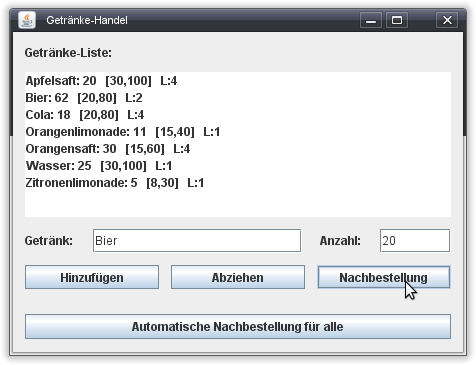
\includegraphics[width=0.85\textwidth]{./inf/SEKII/38_JavaSQL_Wiederholung/GetraenkeHandelAufgabe6.png}
 \caption{Die Programmoberfläche von \glqq Getränke-Handel\grqq}
 \label{fig:getraenkehandel}
\end{figure}

\item Erstelle ein Java-Programm für den Getränkehandel. Abbildung
\ref{fig:getraenkehandel} zeigt, wie die Oberfläche des Programms
aussehen soll.
 
In der Listkomponente werden alle Getränke aufgelistet, die das Geschäft führt. Die Ausgabe der
Getränke-Daten erfolgt nach folgendem Schema:

\verb|name: anzahl   [min_anzahl; max_anzahl]   L:getränk_lieferant_id|

Vor- und nach dem Teil in den eckigen Klammern sollten mehrere Leerzeichen
eingefügt werden, damit die Ausgabe besser lesbar wird. Die Anzeige aller
Getränke in der Listkomponente soll automatisch beim Start des Programms
erfolgen. Außerdem soll die Anzeige nach dem Hinzufügen oder Abziehen von
Getränkekisten aktualisiert werden.

Wenn neue Getränkekisten geliefert wurden, gibt der Benutzer den Namen des
gelieferten Getränkes und die Anzahl der gelieferten Kisten in die Textfelder
ein und drückt auf den Button \myPMI{Hinzufügen}. Das Programm erhöht in der
Datenbank die Anzahl der vorhandenen Kisten um den neuen Wert und aktualisiert
die Ausgabe in der Listkomponente. Es muss nicht überprüft werden, ob die
Benutzereingaben korrekt sind.

Wenn Getränkekisten verkauft wurden, gibt der Benutzer den Namen des verkauften
Getränkes und die Anzahl der verkauften Kisten in die Textfelder ein und drückt
auf den Button \myPMI{Abziehen}. Das Programm erniedrigt in der Datenbank die
Anzahl der vorhandenen Kisten um den angegebenen Wert und aktualisiert die
Ausgabe in der Listkomponente. Es muss nicht überprüft werden, ob die
Benutzereingaben korrekt sind.

Das Programm soll später einmal automatisch Briefe generieren können, in denen
Getränke nachbestellt werden. Da dies nur ein Prototyp ist, werden die „Briefe“
in vereinfachter Form auf der Konsole ausgegeben. Eine Textzeile kannst du mit
dem Kommando \lstinline|System.out.println(...);| auf der Konsole ausgeben.

Wenn der Benutzer auf den Button \myPMI{Nachbestellung} drückt, soll das im
linken Textfeld angegebene Getränk in der im rechten Textfeld stehenden Anzahl
bestellt werden. Die Korrektheit der Benutzereingaben braucht auch hier nicht
überprüft zu werden. Die Ausgabe soll nach folgendem Schema erfolgen:

\texttt{\slshape{firma}\\
\slshape{straße}\\
\slshape{ort}}\\
\texttt{Wir benötigen \slshape{anzahl}} \texttt{Kisten \slshape{getränk}.}

Im abgebildeten Beispiel würde zum Beispiel folgender Text auf der Konsole
ausgegeben werden:

\begin{verbatim}
Brauerei Hansen
Buchenweg 244
10352 Lummerstadt
Wir benötigen 78 Kisten Bier.
\end{verbatim}

Wenn der Benutzer auf den Button \myPMI{Automatische Nachbestellung für alle}
klickt, soll eine automatische Nachbestellung für alle Getränke generiert
werden, deren Anzahl unter den Wert \myUserInput{min\_anzahl} gesunken ist. Die
Ausgabe soll nach dem gleichen Schema wie bei einer manuellen Nachbestellung
erfolgen. Alle Nachbestellungen, die an denselben Lieferanten gehen, sollen in
einem „Brief“ zusammen gefasst werden. Leite die Automatische Nachbestellung
durch einen geeigneten Anfangstext (z.B. “AUTOMATISCHE BESTELLUNG – ANFANG“)
gefolgt von einer Leerzeile ein. Hinter der letzten Bestellung soll zuerst eine
Leerzeile und dann ein End-Text (z.B. “AUTOMATISCHE BESTELLUNG – ENDE“) stehen.
Zwischen zwei Nachbestellungen soll jeweils eine Leerzeile liegen (nicht
mehrere!). Im abgebildeten Beispiel würde die Automatische Nachbestellung
folgendermaßen aussehen:

\pagebreak

\begin{verbatim}
AUTOMATISCHE BESTELLUNG - BEGIN

Limonaden-Mix GmbH
Karl-Hauser-Str. 33-35
32011 Quakenbrück
Wir benötigen 75 Kisten Wasser.
Wir benötigen 29 Kisten Orangenlimonade.
Wir benötigen 25 Kisten Zitronenlimonade.

Brauerei Hansen
Buchenweg 244
10352 Lummerstadt
Wir benötigen 78 Kisten Bier.

Cola und Co. KG
Breitenweg 214-215
88123 Heiligenrode
Wir benötigen 80 Kisten Apfelsaft.
Wir benötigen 62 Kisten Cola.

AUTOMATISCHE BESTELLUNG - ENDE
\end{verbatim}

Um die Nachbestellungen eines Lieferanten zusammenfassen zu können, kannst du
dir der Reihe nach die Daten der Lieferanten mit den Nummern 1 bis 10 holen
(Achtung: nicht alle Nummern sind vergeben!). Wenn ein Lieferant mit der
entsprechenden Nummer existiert, holst du dir die Daten aller Getränke, die von
diesem Lieferanten geliefert werden und überprüfst, ob Nachbestellungen nötig
sind.

Beachte, dass die Anschrift eines Lieferanten nur ausgegeben werden darf, wenn
es auch tatsächlich eine Nachbestellung für den Lieferanten gibt.

Anmerkung: Man kann auch auf das Hochzählen der Lieferanten-Nummer verzichten
und direkt die Liste der vorhandenen Lieferanten durchgehen. Für diese Lösung
muss man jedoch zwei verschiedene \lstinline|SELECT|-Abfragen ineinander
verschachteln. Beachte, dass eine Verschachtelung von zwei verschiedene
Da\-ten\-bank\-ab\-fra\-gen nur möglich ist, wenn man für beide Zugriffe ein
eigenes \myClass{Statement}-Objekt und ein eigenes \myClass{ResultSet}-Objekt erzeugt.
\end{compactenum}
